%==============================================================================
%  Language-Conditioned Robotic Vial Sorting with a Vision-Language-Action Policy
%  Compile in Overleaf:  pdfLaTeX  ->  BibTeX  ->  pdfLaTeX  ->  pdfLaTeX
%  Figures go in the  imgs/  folder (see docs/imgs_links/figures.md for sources).
%==============================================================================
\documentclass[11pt]{article}

\usepackage[margin=1in]{geometry}
\usepackage{graphicx}
\usepackage{amsmath,amssymb}
\usepackage{booktabs}
\usepackage{caption}
\usepackage{subcaption}
\usepackage{xcolor}
\usepackage{float}
\usepackage[numbers,square]{natbib}
\usepackage[hidelinks]{hyperref}

\graphicspath{{imgs/}}
\captionsetup{font=small}

% --- placeholder box for figures not yet added -------------------------------
\newcommand{\figplaceholder}[1]{%
  \fbox{\parbox[c][0.30\textheight][c]{0.92\textwidth}{\centering
  \textcolor{gray}{\textbf{[ FIGURE PLACEHOLDER ]}\\[4pt] #1}}}}

\title{\textbf{Language-Conditioned Robotic Vial Sorting\\with a Vision--Language--Action Policy}}
\author{Sari Abdan}
\date{\today}

\begin{document}
\maketitle

\begin{abstract}
We describe a language-conditioned robotic system that sorts colored laboratory
vials into rack slots or a discard bin from natural-language commands, built on a
low-cost SO-101 six-degree-of-freedom manipulator running on an NVIDIA Jetson Thor
with three RGB cameras. We collect a teleoperated demonstration dataset of $150$
episodes under a controlled scene grammar---colors crossed with destinations,
spaced distractor vials, and held-out slot positions---and use it to fine-tune a
$\pi_{0.5}$ vision--language--action (VLA) flow policy with the vision and language
backbones frozen and only the action expert trained. Commands use a
source-to-destination \emph{position} grammar, so a high-level planner reasons over
object identity while the low-level policy performs spatial pick-and-place. On the
deployed system the policy follows the commanded destination reliably and completes
autonomous rack-to-rack sorts. A checkpoint study identifies the best operating
point, and we analyze grasp reliability across rack positions together with a
demonstration-consistency effect on bin placement.
\end{abstract}

%==============================================================================
\section{Introduction}
%==============================================================================
Repetitive pick-and-place of laboratory consumables---moving vials between racks
and discarding those that do not belong---is a natural target for learned
manipulation. Vision--language--action (VLA) models map camera observations and a
natural-language instruction directly to robot actions \citep{rt2,black2024pi0},
and a hierarchical arrangement, in which a high-level planner issues atomic
instructions to a low-level VLA executor, follows open-ended commands robustly
\citep{shi2025hirobot}. We adopt this arrangement: a planner selects which vial
goes where, and a VLA executor carries out each atomic move.

We built the SO-101 arm and assembled and calibrated the full rig; the data
collection, policy training, and evaluation were carried out collaboratively. This
report covers the hardware and how the arm was built (Section~\ref{sec:setup}); the
client--server architecture and control interface (Section~\ref{sec:arch}); the
teleoperated dataset, its scene grammar and constraints (Section~\ref{sec:data});
the policy and its training regime (Section~\ref{sec:training}); and the deployment
experiments and results (Section~\ref{sec:experiments}).

\begin{figure}[H]
  \centering
  \includegraphics[width=0.9\textwidth]{system_overview.drawio.png}
  \caption{System overview. A high-level planner grounds object identity and emits
  a source-to-destination position command; the low-level VLA policy executes the
  spatial pick-and-place on the SO-101 arm.}
  \label{fig:overview}
\end{figure}

%==============================================================================
\section{System Setup and Assembly}
\label{sec:setup}
%==============================================================================
\paragraph{Building the arm.}
The SO-101 is an open, 3D-printed six-DOF design. We printed the structural parts,
assembled the six Feetech STS3215 serial-bus servomotors into the linkage, and
built a matched pair of arms---a \emph{leader} for teleoperation and a
\emph{follower} that executes---wiring each as a daisy-chained serial bus and
calibrating every joint's range and zero position.

\medskip
The manipulator is an SO-101 six-DOF arm operated in a leader--follower
configuration for teleoperation: a human moves the leader arm and the follower
mirrors it. All computation---camera capture, policy inference, and motor
control---runs on an NVIDIA Jetson Thor. Three cameras record at $640\times480$ and
$30$\,fps: an overhead \emph{top} camera, a \emph{wrist} camera, and a front-facing
Intel RealSense D435i \emph{side} camera.

The workspace holds two six-slot tube racks arranged diagonally to the arm, with a
bin placed to the left for discards (Figure~\ref{fig:setup}). To remove ambiguity,
all spatial references are defined from the side-camera image: the \emph{left} rack
is the one on the left of that image (nearest the bin), the \emph{right} rack is on
the right, and slots are numbered $1$ to $6$ from left to right in the image.
Assembly included mounting and pinning the three cameras, fixing the rack and bin
footprints, calibrating the leader and follower arms, and verifying the serial
motor bus. A safety watchdog monitors per-motor temperature and current and cuts
torque after repeated limit violations.

\paragraph{Sensing.}
The side RealSense additionally provides a metric depth stream, recorded alongside
RGB. Because the vials are transparent glass, active-stereo depth is unreliable on
them, so the policy is trained from the RGB streams.

\begin{figure}[H]
  \centering
  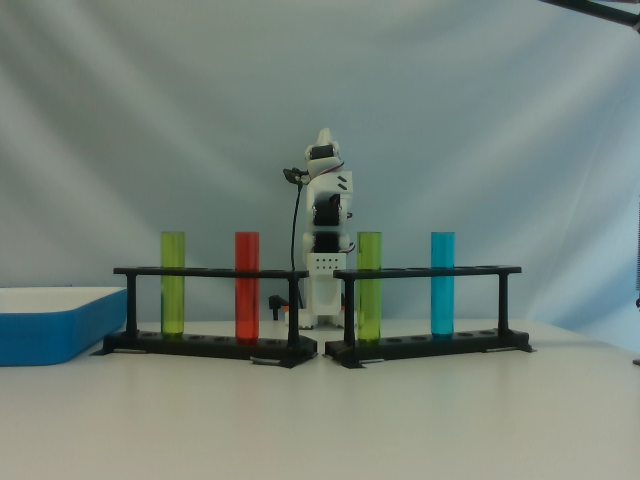
\includegraphics[width=0.8\textwidth]{setup_side.png}
  \caption{The vial-sorting rig, viewed from the side camera. Two six-slot racks
  are arranged diagonally to the arm; the discard bin sits to the left. All
  left/right and slot references in this report are defined from this view.}
  \label{fig:setup}
\end{figure}

\begin{figure}[H]
  \centering
  \includegraphics[width=0.95\textwidth]{imgs/cameras.png}
  \caption{The three camera streams recorded and served to the policy: overhead
  top, wrist, and front-facing side (Intel RealSense D435i).}
  \label{fig:cameras}
\end{figure}

%==============================================================================
\section{System Architecture and Control Interface}
\label{sec:arch}
%==============================================================================
The system follows a client--server design (Figure~\ref{fig:arch}). The robot, the
three cameras, and the policy all reside on the Jetson Thor, wrapped by an inference
server (\texttt{vla\_server.py}) that exposes a small HTTP interface:
\texttt{/execute} runs a commanded move for a fixed duration, \texttt{/home}
returns the arm to the training start pose, \texttt{/observe} and \texttt{/state}
stream the live camera frames and status, and \texttt{/stop} halts motion
immediately. Because every hardware interaction sits behind this interface, any
client can drive the robot without touching the hardware directly.

The operator-facing client is a browser control panel (\texttt{cv\_run.py}) that
runs on the workstation and communicates with the Jetson only over HTTP. It shows
the three live camera feeds, overlays the policy's motion path on each feed as it
moves, and includes a classical computer-vision ``slot reader'' that detects which
vial sits in which slot and pre-builds the corresponding command; Home and Execute
controls issue the matching HTTP calls. The inference server additionally serves a
lightweight built-in dashboard for direct control. A representative interaction is
summarized as a use case in Figure~\ref{fig:usecase}: the operator monitors the
feeds, optionally analyzes the scene, enters a source-to-destination command, homes
the arm, and executes the move, with an emergency stop available at all times.

\begin{figure}[H]
  \centering
  \includegraphics[width=0.95\textwidth]{system_architecture.drawio.png}
  \caption{System architecture. The workstation control panel talks to the
  Jetson-hosted inference server only over HTTP; the server holds the policy, the
  cameras, and the SO-101 arm.}
  \label{fig:arch}
\end{figure}

\begin{figure}[H]
  \centering
  \includegraphics[width=0.7\textwidth]{usecase.drawio.png}
  \caption{Use-case view of the control panel: monitoring, scene analysis, command
  entry, homing, execution, and emergency stop.}
  \label{fig:usecase}
\end{figure}

%==============================================================================
\section{The Vial-Sort Dataset}
\label{sec:data}
%==============================================================================
The core of this work is a teleoperated demonstration dataset recorded with the
LeRobot framework \citep{lerobot}. As the operator drives the leader arm and the
follower mirrors it, every timestep is logged with the three RGB camera streams (a
colorized depth channel is stored alongside), the joint states, and the language
instruction. The dataset contains \textbf{150 demonstrations}, each a single atomic
pick-and-place of roughly $23$\,s ($\sim$700 frames) at $30$\,Hz.

\subsection{Task and scenarios}
Every demonstration realizes one atomic skill: pick a designated \emph{target} vial
from its source slot and place it at a commanded destination---either a slot in one of
the two six-slot racks or the discard bin. Targets appear in three colors (red, cyan,
dark green), and colors are \emph{fully crossed} with destinations: every color is
demonstrated to every destination. Each scene additionally holds two to four
\emph{distractor} vials of other colors, so the policy must localize the commanded
slot in clutter rather than reach for the only object present.

\subsection{Constraints}
\label{sec:constraints}
Scenes are generated from a fixed, seeded layout sheet under a set of constraints,
each chosen for a concrete reason---to keep every episode physically executable, to
keep the target unambiguous, and to turn the layout into a controlled test of
generalization. The resulting composition is summarized in Table~\ref{tab:dataset}.

\begin{itemize}\itemsep3pt
  \item \textbf{Spacing --- no two vials in adjacent slots.} The parallel-jaw gripper
  needs finger clearance on \emph{both} sides of a vial; an immediate neighbor blocks
  the grasp and the release. Enforcing spacing on the target \emph{and} every
  distractor keeps every vial pickable and every slot droppable.
  \item \textbf{Destination clearance --- empty slot, both neighbors free.} A release
  into a slot needs room on either side; in practice leaving only \emph{one} neighbor
  free was not enough, so the destination and both its neighbors are kept empty, and
  the target never starts adjacent to its destination.
  \item \textbf{Capacity and stock --- $\le 3$ vials per rack, $\le 3$ of any color.}
  Three vials per rack make the scene look realistically full without becoming
  infeasible to service; the per-color cap matches the physical stock of three vials
  per color.
  \item \textbf{Color set --- three distinct colors, distractors never the target
  color.} Restricting to three well-separated colors (red, cyan, dark green) yields
  denser demonstrations per color and unambiguous grounding, and because distractors
  are never the target's color, the target is the unique vial of its color in the
  scene.
  \item \textbf{Held-out positions.} Targets originate only from slots $\{1,3,4,6\}$
  and trained destinations are only $\{1,3,6\}$; slots $\{2,4,5\}$ are never used in
  training and are reserved to test interpolation to unseen positions at evaluation.
  \item \textbf{Full crossing.} Because every color is paired with every destination,
  no color is correlated with a fixed slot; the \emph{instruction}, not a memorized
  color-to-slot shortcut, must determine where the vial goes.
\end{itemize}

\paragraph{Fixed objects are constraints too.}
The cameras, the two racks, and the bin are all held in fixed positions, and the
entire left/right/slot naming convention is read off the fixed side-camera image
(Figure~\ref{fig:scene}). This is not incidental: the spatial grammar only means
something if the viewpoint that defines it does not move.

\paragraph{Why a fixed camera.}
A fixed camera maps each physical slot to the \emph{same} region of the image in
every episode, so the policy can reliably associate ``slot~$n$'' with a stable visual
location. A camera that drifts or is repositioned shifts the whole observation
distribution, and a policy trained under one viewpoint degrades under another. We saw
this directly: when the top camera drifted from its mounted pose, a $\pi_0$ policy
that had previously worked stopped working---its inputs had moved outside the
distribution it was trained on. We therefore keep the rig rigid and re-anchor each
camera to a saved reference frame before recording, treating viewpoint stability as a
first-class data constraint.

\begin{figure}[H]
  \centering
  \includegraphics[width=0.85\textwidth]{scene_example.drawio.png}
  \caption{An example scene under the constraints. The starred vial is the
  \emph{target}; distractors are spaced so no two vials are adjacent; the destination
  slot is empty with both neighbors free; slots $\{2,4,5\}$ (shaded) are held out of
  training. Left/right and slot numbers are read from the fixed side-camera view.}
  \label{fig:scene}
\end{figure}

\subsection{Prompt design}
Commands use a source-to-destination \emph{position} grammar---e.g. \emph{``Move the
vial from position 3 of the left rack to slot 6 of the right rack''} or \emph{``\ldots
to the bin''}---and the color of the vial is deliberately never named. Addressing the
source slot keeps the instruction unambiguous even when several vials share a color:
the high-level planner performs the color-to-position grounding, and the low-level
executor performs a purely spatial pick-and-place, mirroring the high-level/low-level
split of hierarchical VLAs \citep{shi2025hirobot}.

A single command is realized under a large space of surface forms. Every instruction
is composed from independent pools---the verb, the object noun, the phrasing of each
slot, the phrasing of each rack, the phrasing of the bin, and the sentence
template---listed in Table~\ref{tab:prompts}. Multiplying these out gives on the order
of $6\times4\times(5\times4)\times(5\times4)\times4\approx 3.8\times10^{4}$ distinct
phrasings of a single rack-to-rack command (about $10^{4}$ for the bin variant). The
dataset draws from this space deterministically, so consecutive demonstrations of the
\emph{same} underlying command are phrased differently; this forces the policy to
parse the language rather than latch onto one fixed template. Table~\ref{tab:examples}
shows representative realizations.

\begin{table}[H]
  \centering
  \caption{Prompt-design pools. Each instruction is one draw from each row.}
  \label{tab:prompts}
  \begin{tabular}{l p{0.66\textwidth}}
    \toprule
    \textbf{Dimension} & \textbf{Values} \\
    \midrule
    Verb (6)          & Move, Take, Transfer, Bring, Relocate, Carry \\
    Object noun (4)   & the vial, the tube, the test tube, the sample tube \\
    Slot phrasing (5) & position~$n$, slot~$n$, the $n$th slot, hole~$n$, spot~$n$ \\
    Rack phrasing (4) & the left rack, the rack on the left, the left-side rack, the left tube rack \\
    Bin phrasing (5)  & the bin, the trash, the waste bin, the trash can, the rubbish bin \\
    Template (4)      & ``\ldots from $S$ to $D$'', ``\ldots in $S$ to $D$'', ``\ldots from $S$ over to $D$'', ``\ldots at $S$ to/into $D$'' \\
    \bottomrule
  \end{tabular}
\end{table}

\begin{table}[H]
  \centering
  \caption{Example prompts drawn from the pools of Table~\ref{tab:prompts}.}
  \label{tab:examples}
  \begin{tabular}{p{0.92\textwidth}}
    \toprule
    \emph{Move the vial from position 3 of the left rack to slot 6 of the right rack.} \\
    \emph{Take the tube in slot 3 of the rack on the left to the sixth slot of the right rack.} \\
    \emph{Transfer the test tube from the third slot of the left-side rack over to hole 6 of the right tube rack.} \\
    \emph{Bring the sample tube at spot 1 of the left tube rack to position 3 of the right rack.} \\
    \emph{Relocate the vial from hole 4 of the right rack to the first slot of the left rack.} \\
    \emph{Carry the tube from position 6 of the right-side rack to slot 1 of the left rack.} \\
    \emph{Move the test tube from position 4 of the right rack to the trash can.} \\
    \emph{Take the sample tube in slot 1 of the left rack into the waste bin.} \\
    \bottomrule
  \end{tabular}
\end{table}

\subsection{Recording and data fields}
\paragraph{Representation.}
Actions and proprioceptive state are expressed in the end-effector frame: recorded
joint positions are mapped to a seven-dimensional end-effector pose (position,
orientation, gripper) by forward kinematics from the arm's URDF.

\paragraph{Recording and coverage.}
Demonstrations were recorded in short runs that share a single command, against a
deterministic, seeded scene sheet. The sheet balances coverage so that every
(color, destination) pairing appears a similar number of times and no single layout
is over-represented. The arm returns to a common home pose before each episode, with
a brief reset interval between recordings. Instructions were authored
programmatically and expanded into many surface forms per pairing---varying the verb,
the slot phrasing, and the rack phrasing---so the policy sees diverse language for the
same underlying command.

\paragraph{Data fields.}
Following the LeRobot dataset layout, each timestep stores the three RGB images
(\texttt{top}, \texttt{wrist}, \texttt{side}) and a colorized depth image, a
seven-dimensional end-effector state (\texttt{observation.state}), the
seven-dimensional end-effector action (\texttt{action}), the natural-language task
string, and episode/frame indices.

\begin{table}[H]
  \centering
  \caption{Composition of the vial-sort dataset.}
  \label{tab:dataset}
  \begin{tabular}{ll}
    \toprule
    \textbf{Property} & \textbf{Value} \\
    \midrule
    Demonstrations         & 150 (one atomic pick-and-place each) \\
    Frame rate / length    & $30$\,Hz, $\sim$23\,s ($\sim$700 frames) per episode \\
    Modalities             & 3 RGB cameras (top, wrist, side); colorized depth stored \\
    Colors                 & red, cyan, dark green \\
    Racks / slots          & 2 racks $\times$ 6 slots, plus a discard bin \\
    Destinations           & rack slots $\{1,3,6\}$ (left/right) + bin, crossed with color \\
    Source slots           & $\{1,3,4,6\}$ \\
    Held-out slots         & $\{2,4,5\}$ (interpolation test) \\
    Distractors per scene  & 2--4, spaced, never the target color \\
    Per-rack capacity      & $\le 3$ vials; $\le 3$ of any color \\
    Command grammar        & source $\rightarrow$ destination, paraphrased \\
    Action / state         & 7-D end-effector (padded to 32) \\
    \bottomrule
  \end{tabular}
\end{table}

\begin{figure}[H]
  \centering
  \includegraphics[width=0.95\textwidth]{imgs/teleop_dataset.png}
  \caption{A recorded demonstration replayed with every camera view, the joint
  trajectory, and the language instruction synchronized on a single timeline---the
  format the policy is trained on.}
  \label{fig:dataset}
\end{figure}

%==============================================================================
\section{Policy Learning}
\label{sec:training}
%==============================================================================
The policy is $\pi_{0.5}$ \citep{pi05}, a vision--language--action flow model of
roughly three billion parameters in the $\pi_0$ family \citep{black2024pi0},
fine-tuned from the released base weights. We train in a \emph{frozen} regime: the
vision encoder and the vision--language backbone are held fixed and only the action
expert---the flow-matching head that produces motions---is updated.

\paragraph{Why freeze.}
With only $150$ demonstrations, updating billions of vision parameters overfits the
recorded scenes and erodes the pretrained language grounding that makes the model
follow instructions; freezing preserves those priors and regularizes the small-data
regime, the standard transfer-learning outcome for VLAs \citep{rt2,openvla}.
Training such a model from scratch is infeasible at this data scale. The choice is
empirical as well: an unfrozen variant of the comparison model overfit and failed
to grasp, while the frozen policy trained cleanly. Table~\ref{tab:config} lists the
configuration.

\begin{table}[H]
  \centering
  \caption{Training configuration for the deployed $\pi_{0.5}$ policy.}
  \label{tab:config}
  \begin{tabular}{ll}
    \toprule
    \textbf{Setting} & \textbf{Value} \\
    \midrule
    Base model            & $\pi_{0.5}$ pretrained base \\
    Trainable parameters  & action expert only (vision + VLM frozen) \\
    Precision             & bfloat16 \\
    Learning rate         & $1\times10^{-4}$ \\
    Batch size            & 16 \\
    Steps                 & 30{,}000 (checkpoint every 2{,}000) \\
    Action chunk          & 50 \\
    Action / state space  & 7-D end-effector (padded to 32) \\
    Image augmentation    & enabled \\
    Cameras               & RGB (top, wrist, side) \\
    \bottomrule
  \end{tabular}
\end{table}

\paragraph{Hardware.}
Training ran on a single NVIDIA RTX PRO 6000 Blackwell (96\,GB). Because only the
action expert receives gradients, the frozen regime used roughly $19$\,GB---far
below a full fine-tune---since the frozen majority of the network performs only a
forward pass with no gradient, optimizer, or activation memory.

\paragraph{Comparisons.}
Alongside $\pi_{0.5}$ we trained three other policies on this platform. GR00T~N1.5
\citep{groot2025} was fine-tuned with a frozen visual backbone as an architectural
comparison. A $\pi_0$ model \citep{black2024pi0} was trained on a narrower,
\emph{single-task} scenario---one fixed color-and-destination pairing rather than the
full crossed set of colors and destinations---to probe how well the family grasps
when specialized. In that setting $\pi_0$ produced the strongest grasping we
observed, matching or slightly exceeding $\pi_{0.5}$; however, because it was tied to
that one task and did not follow arbitrary commands across the crossed dataset,
$\pi_{0.5}$---which does---was retained for the deployed, general system. An Action
Chunking Transformer (ACT) \citep{act} was trained as a non-language-conditioned
baseline: it reproduces a single learned motion and does not respond to the command,
but confirms that the autonomous pipeline drives several policy classes.

%==============================================================================
\section{Experiments and Results}
\label{sec:experiments}
%==============================================================================
\paragraph{Deployment.}
A chosen checkpoint is served on the Jetson by an inference server that exposes a
browser control panel with the three live camera feeds and Home/Execute controls
(Figure~\ref{fig:dashboard}). Before every command the arm homes to the start pose
of the demonstrations; we found that a mismatch here produced an
out-of-distribution transient (the arm flailed before recovering) and corrected it
by setting the home pose directly from the recorded data.

\begin{figure}[H]
  \centering
  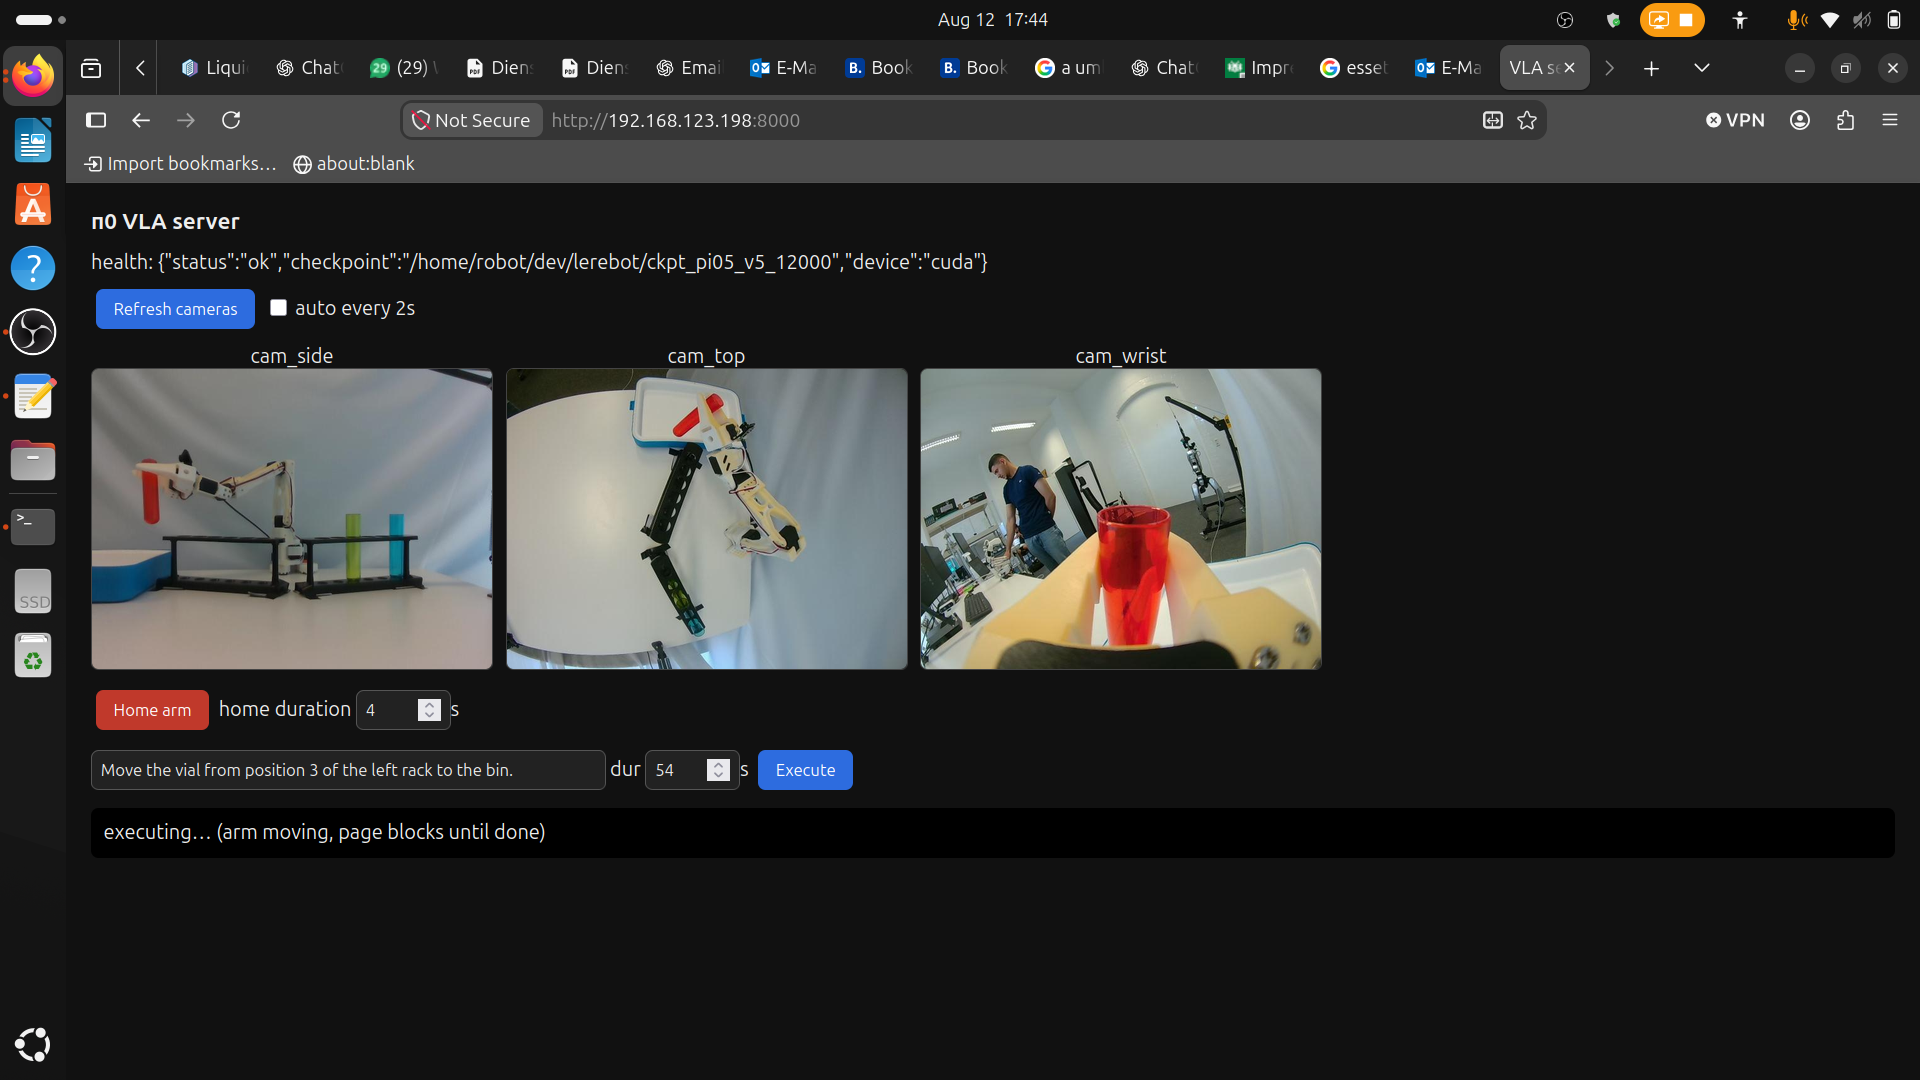
\includegraphics[width=0.95\textwidth]{dashboard.png}
  \caption{The deployment control panel. The three camera feeds are shown live; a
  position command is entered and executed on the arm, which first homes to the
  training start pose.}
  \label{fig:dashboard}
\end{figure}

\paragraph{Checkpoint study.}
Table~\ref{tab:ckpt} summarizes the behavior across training checkpoints. At $8$k
steps the policy does not yet follow the command (its language grounding is
under-trained); at $12$k it follows commands, grasps, and completes placements; at
$16$k it over-fits and loses the grasp. This is the expected
data-density/over-fitting curve, and $12$k is the operating point we deploy.

\begin{table}[H]
  \centering
  \caption{Checkpoint study for the $\pi_{0.5}$ policy. The $12$k checkpoint is the
  deployed operating point.}
  \label{tab:ckpt}
  \begin{tabular}{lccc}
    \toprule
    \textbf{Checkpoint} & \textbf{Follows command} & \textbf{Grasps} & \textbf{Completes rack placement} \\
    \midrule
    8k   & no  & --  & -- \\
    \textbf{12k}  & \textbf{yes} & \textbf{yes} & \textbf{yes} \\
    16k  & yes & no  & no \\
    \bottomrule
  \end{tabular}
\end{table}

\paragraph{Command following.}
We verify instruction following by holding the scene fixed and changing only the
destination clause of the command; the arm then proceeds to different targets
accordingly. Across trials the deployed policy follows the commanded
source-to-destination move reliably.

\paragraph{Grasping and placement.}
Grasping is reliable at the central slot. The two outermost slots ($1$ and $6$) lie
at the extremes of the arm's reach and are harder to grasp cleanly. Rack-to-rack
placement completes end to end: the policy lowers the vial into the target slot and
releases it, yielding a complete autonomous sort (Figure~\ref{fig:racksort}).

\paragraph{Model comparison.}
Across policies, $\pi_0$---in its single-task setting---delivered the most reliable
grasps, slightly ahead of $\pi_{0.5}$, while
$\pi_{0.5}$ followed the source-to-destination instruction most reliably and was
therefore selected for deployment. The ACT baseline reproduced the motion but,
being non-language-conditioned, did not respond to the command.

\begin{figure}[H]
  \centering
  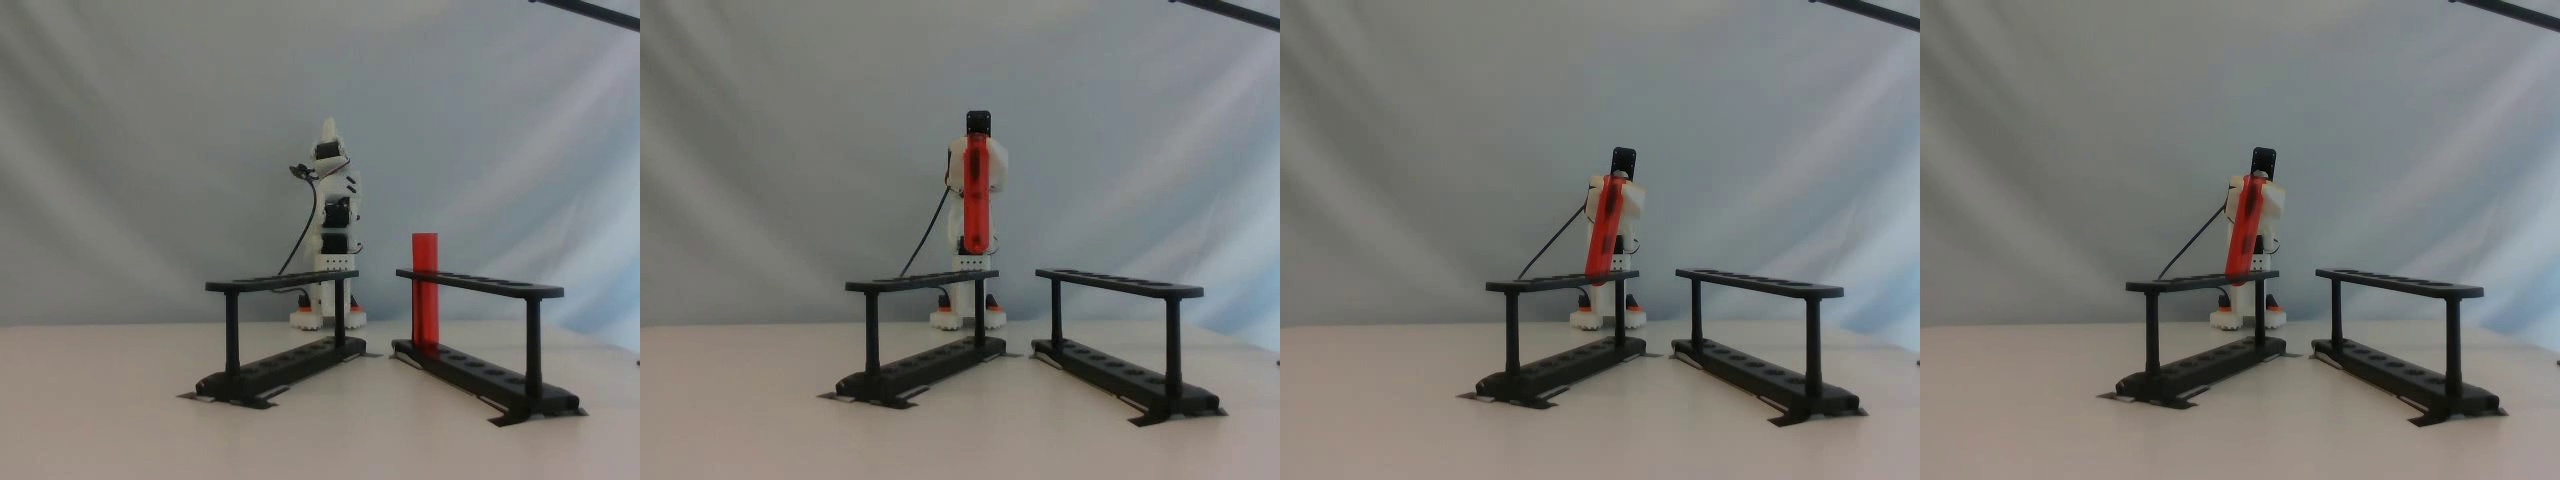
\includegraphics[width=0.98\textwidth]{rack_sort_sequence.png}
  \caption{A complete autonomous rack-to-rack sort under a single position command:
  approach, grasp at the source slot, transport, and release into the destination
  slot.}
  \label{fig:racksort}
\end{figure}

\paragraph{Bin placement.}
For discard commands the arm carries the vial over the bin but does not release it.
This behavior persists across the $8$k, $12$k, and $16$k checkpoints and is
therefore not a training-duration effect. It traces to demonstration inconsistency:
the bin was demonstrated as varied throws, and imitation learning averages
inconsistent demonstrations into a non-committal hover; the bin's location at the
workspace extreme compounds the difficulty. A small set of \emph{consistent}
bin-release demonstrations addresses the behavior.

\paragraph{Discussion.}
The observed grasp and placement behavior is consistent with the known relationship
between demonstration count and success for SO-101-class manipulators: reliability
at a given source/destination scales with the density of demonstrations covering
it, which explains both the strong central-slot behavior and the weaker extremes.
The checkpoint study reproduces the standard trade-off between under-fit language
grounding and over-fit motor behavior, with a clear intermediate optimum.

\bibliographystyle{plainnat}
\bibliography{references}

\end{document}
